\newpage
\section{Theoretical Analysis}
\label{sec:analysis}

\subsection{Mesh Analysis}

%---------------Mesh Analysis--------------------------------------------------------%
\label{sec:Mesh Analysis}
\begin{figure}[!ht] \centering
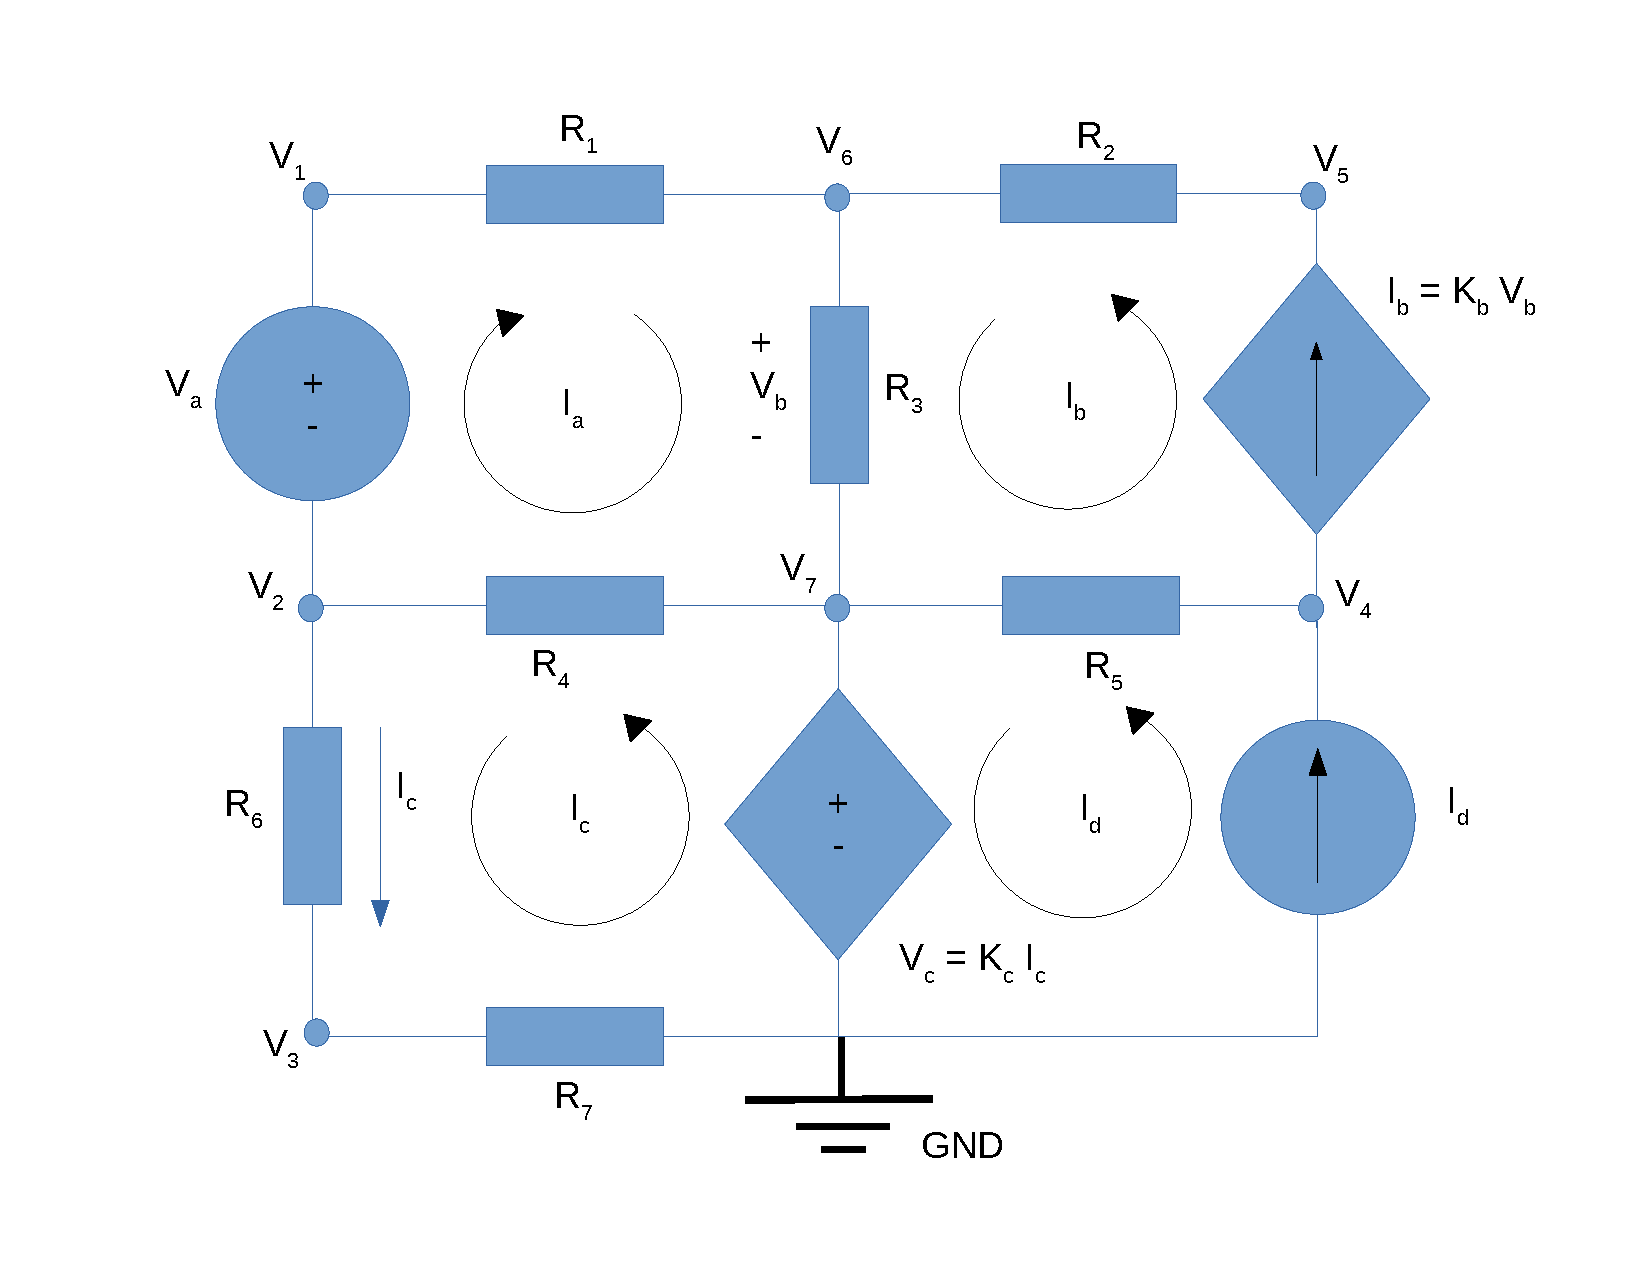
\includegraphics[width=0.8\linewidth]{circuit_mesh.pdf}
\caption{Representation of mesh currents in the circuit.}
\label{fig:meshcurrents}
\end{figure}

Figure~\ref{fig:meshcurrents} shows the mesh currents considered for the circuit analysis, with the current $I_a$ flowing clockwise and the rest of the currents ($I_b$, $I_c$ and $I_d$) flowing counter-clockwise. In the meshes containing $I_b$ and $I_d$, the currents were considered to be the same as the current sources in said meshes.

From this circuit, there can then be extracted 3 equations to figure out the value of the components necessary for the circuit analysis.

The first one, Equation~\ref{eq:meshb}, was obtained by using Ohm's Law, assuming it is known the value of the voltage and the resistance in resistor 3 and that the current flowing through it is ($I_a$ + $I_b$).
\begin{equation}
  I_{b} = K_{b}(I_{a} + I_{b})R_{3},
  \label{eq:meshb}
\end{equation}

Equation~\ref{eq:mesha}  was figured out by analysing the top left mesh, using Kirchoff's Voltage Law and Ohm's Law for the resistors. Since the current $I_a$ is flowing clockwise, the voltage in $V_a$ is negative and the currents in resistors 3 and 4 are, 
correspondingly, ($I_a$ + $I_b$) and ($I_a$ + $I_c$), as these pairs of currents are flowing the same way in said resistors.
\begin{equation}
  -V_{a} + I_{a}R_{1} + (I_{a} + I_{b})R_{3} + (I_{a} + I_{c})R_{4} = 0,
  \label{eq:mesha}
\end{equation}

Finally, from the bottom left mesh, there is Equation~\ref{eq:meshc}, in which was also used Kirchoff's Voltage Law and Ohm's Law. The voltage in $V_c$ is negative due to the current flow.
\begin{equation}
  -K_{c}I_{c} + I_{c}R_{6} + I_{c}R_{7} + (I_{a} + I_{c})R_{4} = 0,
  \label{eq:meshc}
\end{equation}
\newpage

By developing these 3 equations, the matrix below (\ref{eq:matrix}) is achieved as to simplify the calculations. This matrix was solved in Octave, getting the values of the currents $I_a$, $I_b$ and $I_c$ that can be found in table~\ref{table:nodesmesh}. It was not necessary to solve for the value of the current in the bottom right mesh since it is already known (equivalent to $I_d$).

\begin{equation}
\left[ \begin{array}{ccc} -K_bR_3 & 1-K_bR_3 & 0 \\ R_1+R_3+R_4 & R_3 & R_4 \\ R_4 & 0 & R_6+R_7-K_c+R_4 \end{array} \right]
\times \left[ \begin{array}{c} I_a \\ I_b \\ I_c \end{array} \right] =
\left[ \begin{array}{c} 0 \\ V_a \\ 0 \end{array} \right]
\label{eq:matrix}
\end{equation}

With these currents, it is possible to discover the values of the voltages in each node, using the equations~\ref{eq:node7} through~\ref{eq:node1} down below and knowing that $I_b$ = $K_b$$V_b$ and $V_c$=$K_c$$I_c$.
\begin{equation}
  V_{7} = V_{c},
  \label{eq:node7}
\end{equation}

\begin{equation}
  V_{6} = V_{7} + V_{b},
  \label{eq:node6}
\end{equation}

\begin{equation}
  V_{5} = V_{6} + R_{2}I_{b},
  \label{eq:node5}
\end{equation}

\begin{equation}
  V_{4} = V_{7} + R_{5}(I_{d} - I_{b}),
  \label{eq:node4}
\end{equation}

\begin{equation}
  V_{3} = V_{0} + R_{7}I_{c},
  \label{eq:node3}
\end{equation}

\begin{equation}
  V_{2} = V_{3} + R_{6}I_{c},
  \label{eq:node2}
\end{equation}

\begin{equation}
  V_{1} = V_{2} + V_{a},
  \label{eq:node1}
\end{equation}

Table~\ref{table:nodesmesh} shows the nodes' voltages discovered by replacing the known variables in equations~\ref{eq:node7} to ~\ref{eq:node1}. The branch currents were obtained with the following equations~\ref{eq:branch1} to ~\ref{eq:branch6/7} (resorting to figure~\ref{fig:meshcurrents}).

\begin{equation}
  R_1[i] = I_a,
  \label{eq:branch1}
\end{equation}

\begin{equation}
  R_2[i]= I_b,
  \label{eq:branch2}
\end{equation}

\begin{equation}
  R_3[i] = I_a + I_b,
  \label{eq:branch3}
\end{equation}

\begin{equation}
  R_4[i] = I_a + I_c,
  \label{eq:branch4}
\end{equation}

\begin{equation}
  R_5[i] = Id - Ib,
  \label{eq:branch5}
\end{equation}

\begin{equation}
  R_6[i] = R_7[i] = I_c,
  \label{eq:branch6/7}
\end{equation}



\begin{table}[!ht]
\centering
\begin{tabular}{ |c|c|} 
 \hline
 {\bf Node} & {\bf Voltage[V]} \\ 
 \hline\hline
  $V_b$ & \partialinput{1}{1}{malhas.tex}\\ 
 \hline
  $V_c$ & \partialinput{2}{2}{malhas.tex} \\ 
 \hline
 $V_1$ & \partialinput{3}{3}{malhas.tex} \\ 
 \hline
 $V_2$ & \partialinput{4}{4}{malhas.tex} \\ 
 \hline
 $V_3$ & \partialinput{5}{5}{malhas.tex} \\ 
 \hline
 $V_4$ & \partialinput{6}{6}{malhas.tex} \\ 
 \hline
 $V_5$ & \partialinput{7}{7}{malhas.tex} \\ 
\hline
 $V_6$ & \partialinput{8}{8}{malhas.tex} \\ 
 \hline
 $V_7$ & \partialinput{9}{9}{malhas.tex} \\
 \hline
\end{tabular}
\begin{tabular}{ |c|c|} 
 \hline
 {\bf Branch} & {\bf Current[A]}\\ 
 \hline\hline
 $I_b$ & \partialinput{10}{10}{malhas.tex} \\ 
 \hline
 $I_c$ & \partialinput{11}{11}{malhas.tex} \\
 \hline
 $R_1=I_a$ & \partialinput{12}{12}{malhas.tex} \\ 
 \hline
  $R_2$ & \partialinput{13}{13}{malhas.tex} \\ 
 \hline
  $R_3$ & \partialinput{14}{14}{malhas.tex} \\  
 \hline
 $R_4$ & \partialinput{15}{15}{malhas.tex} \\ 
 \hline
 $R_5$ & \partialinput{16}{16}{malhas.tex} \\  
 \hline
 $R_6$ & \partialinput{17}{17}{malhas.tex} \\ 
 \hline
  $R_7$ & \partialinput{18}{18}{malhas.tex} \\  
 \hline
\end{tabular}
\caption{Voltage and Current values using the mesh analysis.}
\label{table:nodesmesh}
\end{table}






\newpage

%---------------Nodal Analysis--------------------------------------------------------%
\subsection{Nodal Analysis}
\label{sec:Nodal Analysis}

\begin{figure}[!ht] \centering
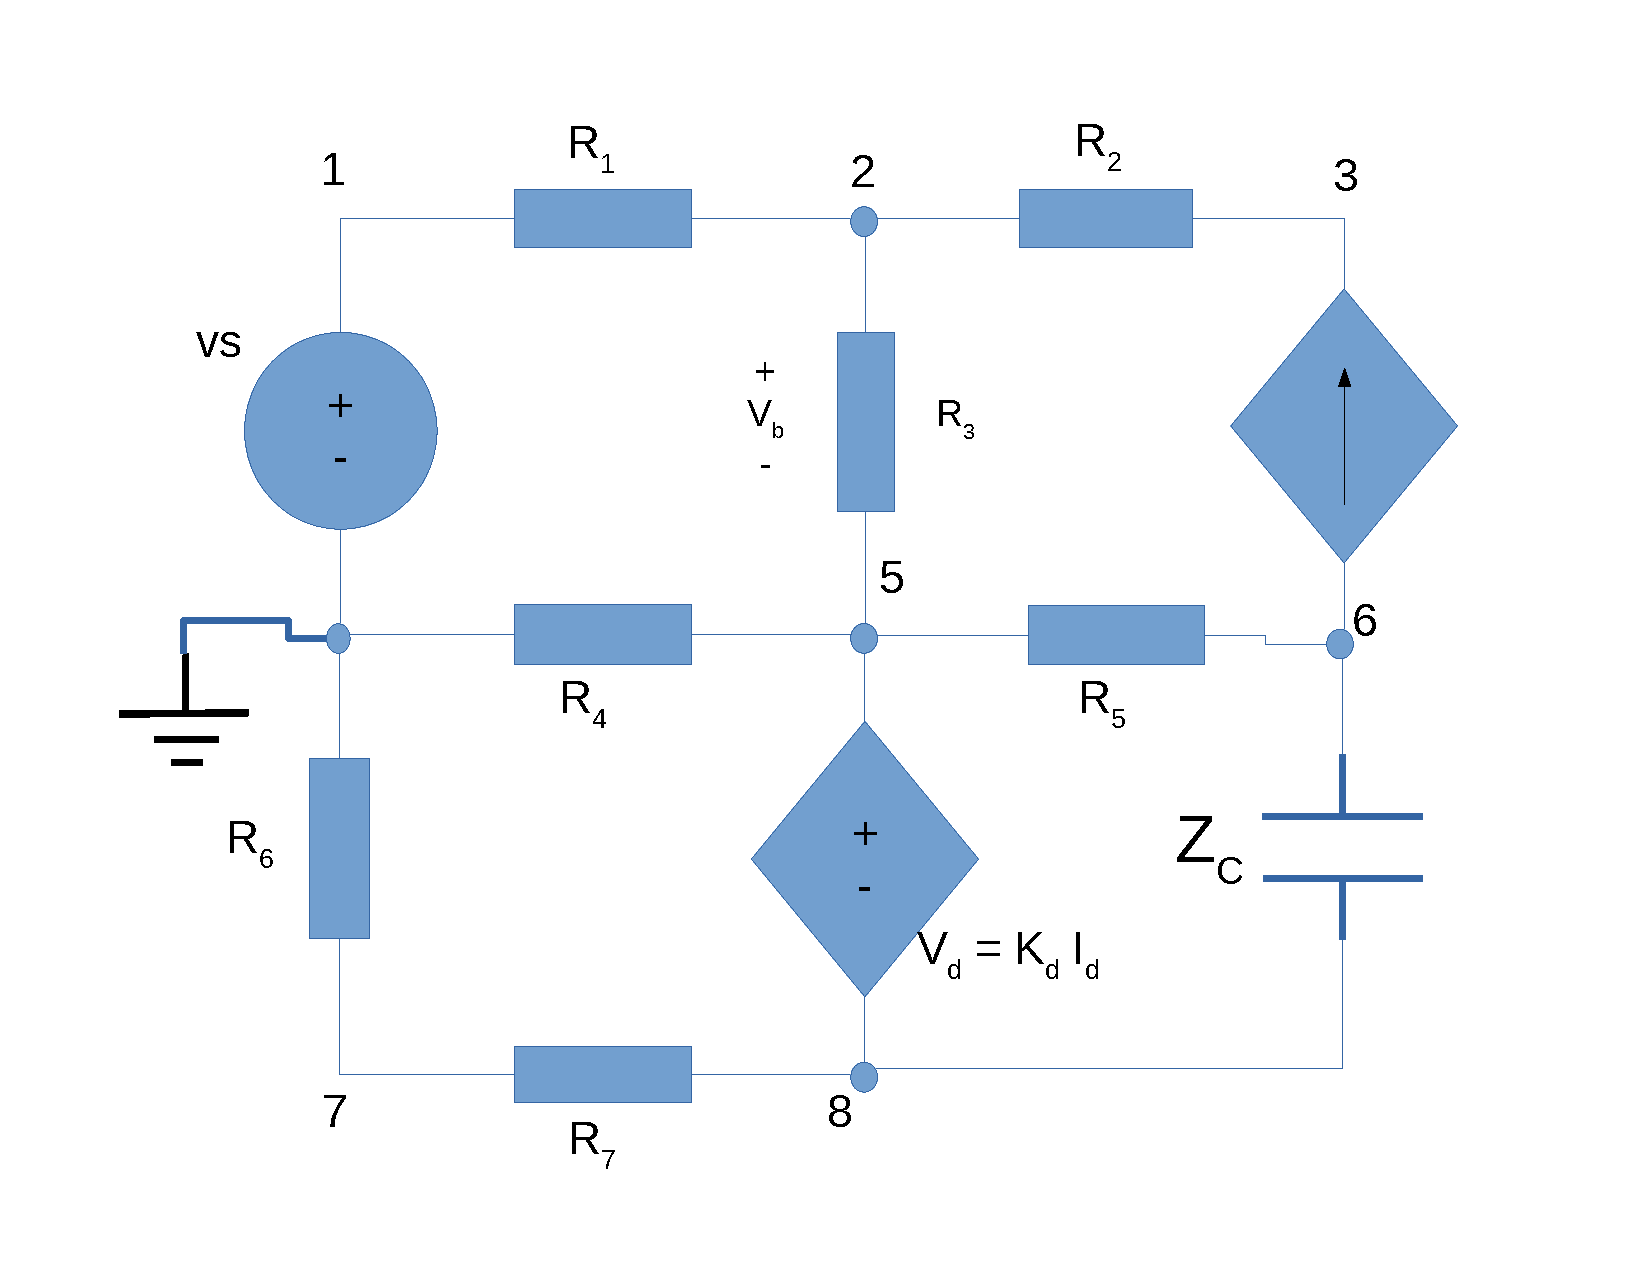
\includegraphics[width=0.8\linewidth]{circuit_node.pdf}
\caption{Representation of the circuit with emphasis on its nodes.}
\label{fig:nodescircuit}
\end{figure}

In order to consistantly analyze this circuit with nodal method, we had figure~\ref{fig:circuit} as a reference to build figure~\ref{fig:nodescircuit}, having considered the same notation for both. In the whole following analysis, we have considered that the current flows according to the direction suggested by the arrow next to each branch. 

The first thing which must be noticed is that there is an independent voltage source ($V_a$) and a linear current controlled voltage source ($V_c$) in this circuit. Knowing that a nodal analysis can't include the analysis of nodes that are connected to voltage sources, it becomes clear that is useless to analyze nodes 1 and 2 (connected to $V_a$) and also nodes 0 and 7 (connected to $V_c$) using this method.

From figure~\ref{fig:nodescircuit}, we can easily conclude that there are 11 unknown variables: $V_b$ $I_b$ $V_c$ $I_c$ $V_1$ $V_2$ $V_3$ $V_4$ $V_5$ $V_6$ $V_7$. If we look at the position we chose for the GND (Ground), we can also infer that value of $V_0$ is 0.

Then, it is mandatory to consider 11 linearly independent equations to reach all the values corresponding to the mentioned variables and consequently solve the circuit. There are 2 equations (given by the Professor - ~\ref{eq:given1} and ~\ref{eq:given2}) explicitly written in figure~\ref{fig:nodescircuit} which are related to the two linear dependent sources:
\begin{equation}
  K_{b}V_{b} - I_{b} = 0,
  \label{eq:given1}
\end{equation}

\begin{equation}
  K_{c}I_{c} - V_{c} = 0,
  \label{eq:given2}
\end{equation}


As referred above, it is possible to use the nodal method to analyze nodes 3, 4, 5 and 6.

Considering the current $I_c$ flowing from node 2 to node 3 and the current passing through $R_7$ diverging from node 3, the equation below (\ref{eq:node3a}) was figured out by using Kirchoff's Current Law for node 3 and Ohm's Law for the resistors $R_6$ and $R_7$. To correctly use the Ohm's Law for the resistor $R_7$, it is important to remember that the value we assigned to $V_0$ is 0.
\begin{equation}
  (V_{2} - V_{3})G_{6} - V_{3}G_{7} = 0,
  \label{eq:node3a}
\end{equation}

The following equation (\ref{eq:node4a}), in which was also used Kirchoff's Current Law and Ohm's Law for resistor $R_4$, refers to node 4. It was considered $I_d$ is converging to the mentioned node, contrarily to $I_b$ and to the current at $R_5$ which are both diverging.
\begin{equation}
  (V_{4} - V_{7})G_{5} + K_{b}V_{b} = I_{d},
  \label{eq:node4a}
\end{equation}

Since $I_b$ is flowing from node 4 to 5 and the current measured at $R_2$ is flowing from node 5 to 6, Kirchoff's Circuit Law (for node 5) and Ohm's Law (for $R_2$) were used to establish the following mathematical relation:
\begin{equation}
  K_{b}V_{b} - (V_{5} - V_{6})G_{2} = 0,
  \label{eq:node5a}
\end{equation}

Considering node 6 as a spatial reference, we assumed there were two divergent currents (one flowing to node 1 and the other to node 7) and a current converging from node 5. Knowing that, the ensuing equation (\ref{eq:node6a}) was figured out by resorting to Ohm's Law for resistors $R_1$, $R_2$ and $R_3$ and Kirchoff's Current Law for node 6. 
\begin{equation}
  K_{b}V_{b} - (V_{6} - V_{1})G_{1} - (V_{6} - V_{7})G_{3} = 0,
  \label{eq:node6a}
\end{equation}

After the previous analysis there are only 6 equations available to work with. This leads us to the inevitability of considering 5 additional equations. 

The equation written below (\ref{eq:add1}) is a direct consequence of our choice of connecting node 0 to the ground (GND), because this choice makes evident that the value of $V_0$ is 0 and then:
\begin{equation}
  V_{7} - V_{c} = 0,
  \label{eq:add1}
\end{equation}

By observing the branches which contain (respectively) the independent voltage source $V_a$ and the linear dependent voltage source $V_c$, it is also trivial that:
\begin{equation}
  V_{1} - V_{2} = V_{a},
  \label{eq:add2}
\end{equation}

\begin{equation}
  V_{b} - V_{6} + V_{7} = 0,
  \label{eq:add3}
\end{equation}

It is mandatory to relate $I_c$ with other unknown variables. So, this equation (\ref{eq:add4}) was obtained by looking at the bottom left mesh and using Ohm's Law for resistor $R_7$.
\begin{equation}
  V_{3}G_{7} - I_{c} = 0,
  \label{eq:add4}
\end{equation}

Ultimately, to discover the last equation, there are some theoretical concepts that must be considered. 

Kirchoff's Current Law implies that there is no current stuck at any node. It is also known that neither voltage sources nor resistors retain current. Then, any branch that only contains one of the said elements does not retain current as well. Merging the two branches placed on the left side of circuit (branch containing $V_a$ with branch containing $R_6$) and calling Supernode to the result of this merger, it is still true that no current is retained in the Supernode. Then, considering that there is current converging from node 6 and assuming that current is diverging from Supernode to nodes 0 and 7, the resultant equation (\ref{eq:supernode}) is the one written right below.
\begin{equation}
  (V_{2} - V_{7})G_{4} + V_{3}G_{7} - (V_{6} - V_{1})G_{1} = 0,
  \label{eq:supernode}
\end{equation}

A system with 11 linearly independent equations and 11 variables is of course possible to solve but not easy (and certainly not pratical) to deal with. The following matrix equation (\ref{eq:nodalmatrix}) summarizes the 11 referred equations so it is easier to read and to instantaneously solve (by using Octave).
\begin{equation}
\left[ \begin{array}{ccccccccccc} 
		K_b & 0 & 0 & 0 & 0 & 0 & 0 & 0 & 0 & -1 & 0 \\ 
		0 & -1 & 0 & 0 & 0 & 0 & 0 & 0 & 0 & 0 & K_c \\
		0 & -1 & 0 & 0 & 0 & 0 & 0 & 0 & 1 & 0 & 0 \\ 
		0 & 0 & 1 & -1 & 0 & 0 & 0 & 0 & 0 & 0 & 0 \\ 
		0 & 0 & 0 & 0 & G_7 & 0 & 0 & 0 & 0 & 0 & -1 \\ 
		1 & 0 & 0 & 0 & 0 & 0 & 0 & -1 & 1 & 0 & 0 \\ 
		0 & 0 & 0 & G_6 & -G_6 - G_7 & 0 & 0 & 0 & 0 & 0 & 0 \\ 
		K_b & 0 & 0 & 0 & 0 & G_5 & 0 & 0 & -G_5 & 0 & 0 \\ 
		K_b & 0 & 0 & 0 & 0 & 0 & -G_2 & G_2 & 0 & 0 & 0 \\ 
		K_b & 0 & G_1 & 0 & 0 & 0 & 0 & -G_1 - G_3 & G_3 & 0 & 0 \\ 
		0 & 0 & G_1 & G_4 & G_7 & 0 & 0 & -G_1 & -G_4 & 0 & 0 
\end{array} \right]
\times \left[ \begin{array}{c} V_b \\ V_c \\ V_1 \\ V_2 \\ V_3 \\ V_4 \\ V_5 \\ V_6 \\ V_7 \\ I_b \\ I_c \end{array} \right] =
\left[ \begin{array}{c} 0 \\ 0 \\ 0 \\ V_a \\ 0 \\ 0 \\ 0 \\ I_d \\ 0 \\ 0 \\ 0 \end{array} \right]
\label{eq:nodalmatrix}
\end{equation}

To find all the required branches' currents we can use Ohm's Law for each resistor, which can be seen in equations~\ref{eq:ohm1} to~\ref{eq:ohm6/7}

\begin{equation}
  R_1[i] = \frac{V_6 - V_1}{R_1},
  \label{eq:ohm1}
\end{equation}

\begin{equation}
  R_2[i]= I_b,
  \label{eq:ohm2}
\end{equation}

\begin{equation}
  R_3[i] = \frac{V_b}{R_3},
  \label{eq:ohm3}
\end{equation}

\begin{equation}
  R_4[i] = \frac{V_2-V_7}{R_4},
  \label{eq:ohm4}
\end{equation}

\begin{equation}
  R_5[i] = \frac{V_4-V_7}{R_5},
  \label{eq:ohm5}
\end{equation}

\begin{equation}
  R_6[i] = R_7[i] = I_c,
  \label{eq:ohm6/7}
\end{equation}

The result of this analysis is reflected in table~\ref{table:nodaltable}, which establishes a mathematical relation between every mentioned variables and its respective values. 

\begin{table}[!ht]
\centering
\begin{tabular}{ |c|c| } 
 \hline
 {\bf Node} & {\bf Voltage[V]} \\ 
 \hline\hline
 $V_b$ & \partialinput{1}{1}{nos.tex} \\ 
 \hline
 $V_c$ & \partialinput{2}{2}{nos.tex} \\ 
 \hline
 $V_1$ & \partialinput{3}{3}{nos.tex} \\ 
 \hline
 $V_2$ & \partialinput{4}{4}{nos.tex} \\ 
 \hline
 $V_3$ & \partialinput{5}{5}{nos.tex} \\ 
 \hline
 $V_4$ & \partialinput{6}{6}{nos.tex} \\ 
 \hline
 $V_5$ & \partialinput{7}{7}{nos.tex} \\ 
\hline
 $V_6$ & \partialinput{8}{8}{nos.tex} \\ 
 \hline
 $V_7$ & \partialinput{9}{9}{nos.tex} \\
 \hline
 

\end{tabular}
\begin{tabular}{ |c|c|} 
 \hline
 {\bf Branch} & {\bf Current[A]}\\ 
 \hline\hline
  $I_b$ & \partialinput{10}{10}{nos.tex} \\ 
 \hline
 $I_c$ & \partialinput{11}{11}{nos.tex} \\
 \hline
  $R_1$ & \partialinput{12}{12}{nos.tex} \\ 
 \hline
  $R_2$ & \partialinput{13}{13}{nos.tex} \\ 
 \hline
  $R_3$ & \partialinput{14}{14}{nos.tex} \\  
 \hline
 $R_4$ & \partialinput{15}{15}{nos.tex} \\ 
 \hline
 $R_5$ & \partialinput{16}{16}{nos.tex} \\  
 \hline
 $R_6$ & \partialinput{17}{17}{nos.tex} \\ 
 \hline
  $R_7$ & \partialinput{18}{18}{nos.tex} \\  
 \hline
\end{tabular}
\caption{Voltage and Current values using the nodal analysis.}
\label{table:nodaltable}
\end{table}

%\lstinputlisting{nos.tex}
 
